%% Generated by Sphinx.
\def\sphinxdocclass{report}
\documentclass[letterpaper,11pt,english]{sphinxmanual}
\ifdefined\pdfpxdimen
   \let\sphinxpxdimen\pdfpxdimen\else\newdimen\sphinxpxdimen
\fi \sphinxpxdimen=.75bp\relax
\ifdefined\pdfimageresolution
    \pdfimageresolution= \numexpr \dimexpr1in\relax/\sphinxpxdimen\relax
\fi
%% let collapsable pdf bookmarks panel have high depth per default
\PassOptionsToPackage{bookmarksdepth=5}{hyperref}

\PassOptionsToPackage{warn}{textcomp}
\usepackage[utf8]{inputenc}
\ifdefined\DeclareUnicodeCharacter
% support both utf8 and utf8x syntaxes
  \ifdefined\DeclareUnicodeCharacterAsOptional
    \def\sphinxDUC#1{\DeclareUnicodeCharacter{"#1}}
  \else
    \let\sphinxDUC\DeclareUnicodeCharacter
  \fi
  \sphinxDUC{00A0}{\nobreakspace}
  \sphinxDUC{2500}{\sphinxunichar{2500}}
  \sphinxDUC{2502}{\sphinxunichar{2502}}
  \sphinxDUC{2514}{\sphinxunichar{2514}}
  \sphinxDUC{251C}{\sphinxunichar{251C}}
  \sphinxDUC{2572}{\textbackslash}
\fi
\usepackage{cmap}
\usepackage[T1]{fontenc}
\usepackage{amsmath,amssymb,amstext}
\usepackage[english]{babel}



\usepackage{tgtermes}
\usepackage{tgheros}
\renewcommand{\ttdefault}{txtt}



\usepackage[Bjarne]{fncychap}
\usepackage{sphinx}

\fvset{fontsize=auto}
\usepackage{geometry}


% Include hyperref last.
\usepackage{hyperref}
% Fix anchor placement for figures with captions.
\usepackage{hypcap}% it must be loaded after hyperref.
% Set up styles of URL: it should be placed after hyperref.
\urlstyle{same}


\usepackage{sphinxmessages}
\setcounter{tocdepth}{1}


% Jupyter Notebook code cell colors
\definecolor{nbsphinxin}{HTML}{307FC1}
\definecolor{nbsphinxout}{HTML}{BF5B3D}
\definecolor{nbsphinx-code-bg}{HTML}{F5F5F5}
\definecolor{nbsphinx-code-border}{HTML}{E0E0E0}
\definecolor{nbsphinx-stderr}{HTML}{FFDDDD}
% ANSI colors for output streams and traceback highlighting
\definecolor{ansi-black}{HTML}{3E424D}
\definecolor{ansi-black-intense}{HTML}{282C36}
\definecolor{ansi-red}{HTML}{E75C58}
\definecolor{ansi-red-intense}{HTML}{B22B31}
\definecolor{ansi-green}{HTML}{00A250}
\definecolor{ansi-green-intense}{HTML}{007427}
\definecolor{ansi-yellow}{HTML}{DDB62B}
\definecolor{ansi-yellow-intense}{HTML}{B27D12}
\definecolor{ansi-blue}{HTML}{208FFB}
\definecolor{ansi-blue-intense}{HTML}{0065CA}
\definecolor{ansi-magenta}{HTML}{D160C4}
\definecolor{ansi-magenta-intense}{HTML}{A03196}
\definecolor{ansi-cyan}{HTML}{60C6C8}
\definecolor{ansi-cyan-intense}{HTML}{258F8F}
\definecolor{ansi-white}{HTML}{C5C1B4}
\definecolor{ansi-white-intense}{HTML}{A1A6B2}
\definecolor{ansi-default-inverse-fg}{HTML}{FFFFFF}
\definecolor{ansi-default-inverse-bg}{HTML}{000000}

% Define an environment for non-plain-text code cell outputs (e.g. images)
\makeatletter
\newenvironment{nbsphinxfancyoutput}{%
    % Avoid fatal error with framed.sty if graphics too long to fit on one page
    \let\sphinxincludegraphics\nbsphinxincludegraphics
    \nbsphinx@image@maxheight\textheight
    \advance\nbsphinx@image@maxheight -2\fboxsep   % default \fboxsep 3pt
    \advance\nbsphinx@image@maxheight -2\fboxrule  % default \fboxrule 0.4pt
    \advance\nbsphinx@image@maxheight -\baselineskip
\def\nbsphinxfcolorbox{\spx@fcolorbox{nbsphinx-code-border}{white}}%
\def\FrameCommand{\nbsphinxfcolorbox\nbsphinxfancyaddprompt\@empty}%
\def\FirstFrameCommand{\nbsphinxfcolorbox\nbsphinxfancyaddprompt\sphinxVerbatim@Continues}%
\def\MidFrameCommand{\nbsphinxfcolorbox\sphinxVerbatim@Continued\sphinxVerbatim@Continues}%
\def\LastFrameCommand{\nbsphinxfcolorbox\sphinxVerbatim@Continued\@empty}%
\MakeFramed{\advance\hsize-\width\@totalleftmargin\z@\linewidth\hsize\@setminipage}%
\lineskip=1ex\lineskiplimit=1ex\raggedright%
}{\par\unskip\@minipagefalse\endMakeFramed}
\makeatother
\newbox\nbsphinxpromptbox
\def\nbsphinxfancyaddprompt{\ifvoid\nbsphinxpromptbox\else
    \kern\fboxrule\kern\fboxsep
    \copy\nbsphinxpromptbox
    \kern-\ht\nbsphinxpromptbox\kern-\dp\nbsphinxpromptbox
    \kern-\fboxsep\kern-\fboxrule\nointerlineskip
    \fi}
\newlength\nbsphinxcodecellspacing
\setlength{\nbsphinxcodecellspacing}{0pt}

% Define support macros for attaching opening and closing lines to notebooks
\newsavebox\nbsphinxbox
\makeatletter
\newcommand{\nbsphinxstartnotebook}[1]{%
    \par
    % measure needed space
    \setbox\nbsphinxbox\vtop{{#1\par}}
    % reserve some space at bottom of page, else start new page
    \needspace{\dimexpr2.5\baselineskip+\ht\nbsphinxbox+\dp\nbsphinxbox}
    % mimick vertical spacing from \section command
      \addpenalty\@secpenalty
      \@tempskipa 3.5ex \@plus 1ex \@minus .2ex\relax
      \addvspace\@tempskipa
      {\Large\@tempskipa\baselineskip
             \advance\@tempskipa-\prevdepth
             \advance\@tempskipa-\ht\nbsphinxbox
             \ifdim\@tempskipa>\z@
               \vskip \@tempskipa
             \fi}
    \unvbox\nbsphinxbox
    % if notebook starts with a \section, prevent it from adding extra space
    \@nobreaktrue\everypar{\@nobreakfalse\everypar{}}%
    % compensate the parskip which will get inserted by next paragraph
    \nobreak\vskip-\parskip
    % do not break here
    \nobreak
}% end of \nbsphinxstartnotebook

\newcommand{\nbsphinxstopnotebook}[1]{%
    \par
    % measure needed space
    \setbox\nbsphinxbox\vbox{{#1\par}}
    \nobreak % it updates page totals
    \dimen@\pagegoal
    \advance\dimen@-\pagetotal \advance\dimen@-\pagedepth
    \advance\dimen@-\ht\nbsphinxbox \advance\dimen@-\dp\nbsphinxbox
    \ifdim\dimen@<\z@
      % little space left
      \unvbox\nbsphinxbox
      \kern-.8\baselineskip
      \nobreak\vskip\z@\@plus1fil
      \penalty100
      \vskip\z@\@plus-1fil
      \kern.8\baselineskip
    \else
      \unvbox\nbsphinxbox
    \fi
}% end of \nbsphinxstopnotebook

% Ensure height of an included graphics fits in nbsphinxfancyoutput frame
\newdimen\nbsphinx@image@maxheight % set in nbsphinxfancyoutput environment
\newcommand*{\nbsphinxincludegraphics}[2][]{%
    \gdef\spx@includegraphics@options{#1}%
    \setbox\spx@image@box\hbox{\includegraphics[#1,draft]{#2}}%
    \in@false
    \ifdim \wd\spx@image@box>\linewidth
      \g@addto@macro\spx@includegraphics@options{,width=\linewidth}%
      \in@true
    \fi
    % no rotation, no need to worry about depth
    \ifdim \ht\spx@image@box>\nbsphinx@image@maxheight
      \g@addto@macro\spx@includegraphics@options{,height=\nbsphinx@image@maxheight}%
      \in@true
    \fi
    \ifin@
      \g@addto@macro\spx@includegraphics@options{,keepaspectratio}%
    \fi
    \setbox\spx@image@box\box\voidb@x % clear memory
    \expandafter\includegraphics\expandafter[\spx@includegraphics@options]{#2}%
}% end of "\MakeFrame"-safe variant of \sphinxincludegraphics
\makeatother

\makeatletter
\renewcommand*\sphinx@verbatim@nolig@list{\do\'\do\`}
\begingroup
\catcode`'=\active
\let\nbsphinx@noligs\@noligs
\g@addto@macro\nbsphinx@noligs{\let'\PYGZsq}
\endgroup
\makeatother
\renewcommand*\sphinxbreaksbeforeactivelist{\do\<\do\"\do\'}
\renewcommand*\sphinxbreaksafteractivelist{\do\.\do\,\do\:\do\;\do\?\do\!\do\/\do\>\do\-}
\makeatletter
\fvset{codes*=\sphinxbreaksattexescapedchars\do\^\^\let\@noligs\nbsphinx@noligs}
\makeatother


\usepackage{graphicx}
\setlength{\parindent}{0pt}
\setlength{\parskip}{5pt}
\usepackage{textpos}

% use the listings package for code snippets
\usepackage{listings}
\lstset{frame=tb,
  language=Fortran,
  aboveskip=3mm,
  belowskip=3mm,
  showstringspaces=false,
  columns=flexible,
  basicstyle={\small\ttfamily},
  numbers=none,
  numberstyle=\tiny\color{gray},
  keywordstyle=\color{blue},
  commentstyle=\color{dkgreen},
  stringstyle=\color{mauve},
  breaklines=true,
  breakatwhitespace=true,
  tabsize=3
}

\definecolor{dkgreen}{rgb}{0,0.6,0}
\definecolor{gray}{rgb}{0.5,0.5,0.5}
\definecolor{mauve}{rgb}{0.58,0,0.82}

\newcommand{\rayleigh}{\textsc{Rayleigh}}
  

\title{Rayleigh}
\date{Apr 05, 2022}
\release{}
\author{Nick Featherstone}
\newcommand{\sphinxlogo}{\sphinxincludegraphics{rayleigh_manual_image_300dpi.jpeg}\par}
\renewcommand{\releasename}{}
\makeindex
\begin{document}

\pagestyle{empty}

\definecolor{dark_grey}{gray}{0.3}

%LINE 1%
{
\renewcommand{\familydefault}{\sfdefault}

\pagenumbering{gobble}
\begin{center}
\resizebox{\textwidth}{!}{\textcolor{dark_grey}{\fontfamily{\sfdefault}\selectfont
COMPUTATIONAL INFRASTRUCTURE FOR GEODYNAMICS (CIG)
}}

%\hrule

%LINE 2%
\color{dark_grey}
\rule{\textwidth}{2pt}

%LINE 3%
%\color{dark_grey}
% FILL: additional organizations
% e.g.: {\Large Organization 1\\Organization 2}
%{\Large }
\end{center}

%COLOR AND CODENAME BLOCK%
\begin{center}
\resizebox{\textwidth}{!}{\colorbox{orange}{\fontfamily{\rmdefault}\selectfont \textcolor{white} {\Large
\hspace{0.2in}\rayleigh{}\hspace{0.1in}} }}
\end{center}

%MAIN PICTURE%
\begin{textblock*}{0in}(0.0in,0.0in)
\begin{center}
\vspace{3em}
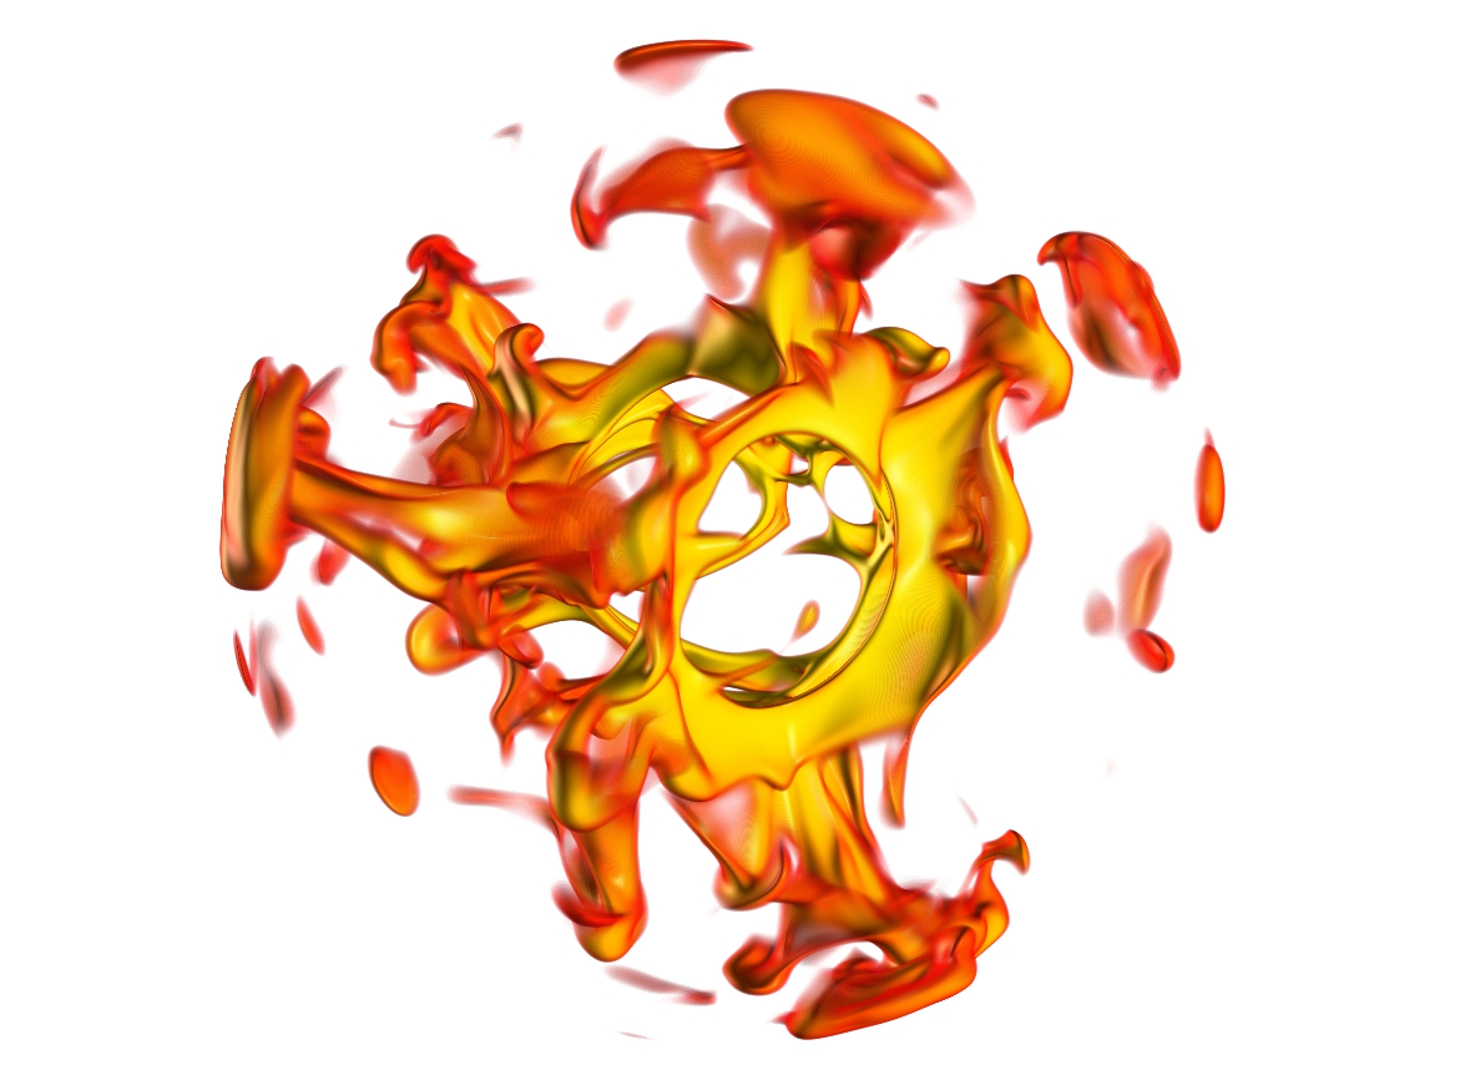
\includegraphics[height=4.0in]
{rayleigh_manual_image_300dpi.jpeg}
\hspace{1em}
\end{center}
\end{textblock*}

%USER MANUAL%
\color{dark_grey}
\vspace{0.5in}
\hfill{\Huge \fontfamily{\sfdefault}\selectfont User Manual \\
\raggedleft \huge \fontfamily{\sfdefault}\selectfont Version
% keep the following line as is so that we can replace this using a script:
1.0.1
\\\large(generated \today)\\
{\Large Nicholas Featherstone\\}
}
%AUTHOR(S) & WEBSITE%
\null
\vspace{17em}
\color{dark_grey}
{\fontfamily{\sfdefault}\selectfont
\large
\vspace{0.3in}
\noindent with contributions by: \\
    Kyle Augustson, Wolfgang Bangerth, Rene Gassm\"oller, Sebastian Glane, Brad Hindman, Lorraine Hwang, Hiro Matsui, Ryan Orvedahl, Krista Soderlund, Cian Wilson, Maria Weber, Rakesh Yadav
    \\
\vspace{1.0em}

{\noindent
{\href{https://geodynamics.org}{geodynamics.org}}
}
}


%LINE%
{\noindent
\color{dark_grey}
\rule{\textwidth}{2pt}
}

%COPYRIGHT STATEMENT
\vspace{-1.5em}
\textcopyright Copyright 2018, Regents of the University of California

}

\pagebreak

\pagestyle{plain}
\sphinxtableofcontents
\pagestyle{normal}
\phantomsection\label{\detokenize{index::doc}}



\chapter{Rayleigh User Manual}
\label{\detokenize{doc/source/Model_Setup/index:rayleigh-user-manual}}\label{\detokenize{doc/source/Model_Setup/index::doc}}

\section{Grid Specification}
\label{\detokenize{doc/source/Model_Setup/grid_specification:grid-specification}}\label{\detokenize{doc/source/Model_Setup/grid_specification::doc}}
\sphinxAtStartPar
Rayleigh solves the fluid equations in spherical\sphinxhyphen{}shell geometry.  As the poles are included, the grid is fully specified by providing four pieces of information:
\begin{itemize}
\item {} 
\sphinxAtStartPar
The coordinates of the computational domain’s radial boundaries of the domain, \(r_\mathrm{min}\) and \(r_\mathrm{max}\)

\item {} 
\sphinxAtStartPar
The number of radial grid points, \(N_r\)

\item {} 
\sphinxAtStartPar
The number of latitudinal grid points, \(N_\theta\)

\end{itemize}

\sphinxAtStartPar
The number of longitudinal grid points, \(N_\phi\) , is always twice \(N_\theta\).
The total number of gridpoints for a Rayleigh simulation is then given by \(2N_rN_\theta^2\).
Note that both \(N_r\) and \(N_\theta\) must be even.   Rayleigh’s computational grid is specified using the problemsize namelist in the main\_input file.
A quick reference for all problemsize\sphinxhyphen{}namelist variables is provided in the {\hyperref[\detokenize{doc/source/Namelist_Definitions/Namelist_Variables:namelists}]{\sphinxcrossref{\DUrole{std,std-ref}{namelist documentation}}}}.  In this section, we discuss in detail how to define
Rayleigh’s grid using these variables.


\subsection{Standard grid specification}
\label{\detokenize{doc/source/Model_Setup/grid_specification:standard-grid-specification}}
\sphinxAtStartPar
We begin by discussing how to define a grid employing a single Chebyshev domain in radius, meaning that a single Chebyshev expansion is carried out over the domain
\(r_\mathrm{min} \le r \le r_\mathrm{max}\).  This is probably the most common grid setup employed in Rayleigh.

\sphinxAtStartPar
The problemsize variables \sphinxstyleemphasis{n\_r} and \sphinxstyleemphasis{n\_theta} provide values
for \(N_r\) and \(N_\theta\) respectively.  Similarly, \sphinxstyleemphasis{rmin} and \sphinxstyleemphasis{rmax} define the value for \(r_\mathrm{min}\) and \sphinxtitleref{r\_mathrm\{max\}}.
If we wanted to define a spherical shell extending from r=1.0 to r=2.0, with \(N_r=48\) and \(N_\theta=96\),
out problemsize namelist should look like:

\begin{sphinxVerbatim}[commandchars=\\\{\}]
\PYG{o}{\PYGZam{}}\PYG{n}{problemsize\PYGZus{}namelist}
 \PYG{n}{n\PYGZus{}r} \PYG{o}{=} \PYG{l+m+mi}{48}
 \PYG{n}{n\PYGZus{}theta} \PYG{o}{=} \PYG{l+m+mi}{96}
 \PYG{n}{rmin} \PYG{o}{=} \PYG{l+m+mf}{1.0}
 \PYG{n}{rmax} \PYG{o}{=} \PYG{l+m+mf}{2.0}
\PYG{o}{/}
\end{sphinxVerbatim}

\sphinxAtStartPar
Note that \(N_r\) and \(N_\theta\) may also be specified at the command
line using the flags \sphinxhyphen{}nr and \sphinxhyphen{}ntheta, e.g.:

\begin{sphinxVerbatim}[commandchars=\\\{\}]
\PYG{n}{mpiexec} \PYG{o}{\PYGZhy{}}\PYG{n}{np} \PYG{l+m+mi}{8} \PYG{o}{.}\PYG{o}{/}\PYG{n}{rayleigh}\PYG{o}{.}\PYG{n}{opt} \PYG{o}{\PYGZhy{}}\PYG{n}{nr} \PYG{l+m+mi}{48} \PYG{o}{\PYGZhy{}}\PYG{n}{ntheta} \PYG{l+m+mi}{96}
\end{sphinxVerbatim}

\sphinxAtStartPar
Doing so will override any values supplied via main\_input.  This can be particularly useful when scripting performance analyses on a new machine.

\sphinxAtStartPar
If desired, a user may instead specify the radial domain bounds in terms of the shell aspect ratio \(\chi=r_\mathrm{min}/r_\mathrm{max}\), and
the shell depth \(r_\mathrm{max}-r_\mathrm{min}\).  This is accomplished using the using the aspect\_ratio and shell\_depth problemsize variables.  The example below describes a
grid equivalent to the one described above.

\begin{sphinxVerbatim}[commandchars=\\\{\}]
\PYG{o}{\PYGZam{}}\PYG{n}{problemsize\PYGZus{}namelist}
 \PYG{n}{n\PYGZus{}r} \PYG{o}{=} \PYG{l+m+mi}{48}
 \PYG{n}{n\PYGZus{}theta} \PYG{o}{=} \PYG{l+m+mi}{96}
 \PYG{n}{aspect\PYGZus{}ratio} \PYG{o}{=} \PYG{l+m+mf}{0.5}
 \PYG{n}{shell\PYGZus{}depth} \PYG{o}{=} \PYG{l+m+mf}{1.0}
\PYG{o}{/}
\end{sphinxVerbatim}

\sphinxAtStartPar
Rayleigh’s horizontal resolution (\(N_\theta\times N_\phi\)) may alternatively be described in terms of spherical harmonics.  The maximum Legendre degree employed in Rayleigh’s truncated spherical harmonic expansion is denoted by \(\ell_\mathrm{max}\), and the total number of degrees by \(N_\ell\).
These two variables are related to \(N_\theta\) via
\begin{equation*}
\begin{split}N_\ell = \ell_\mathrm{max}+1 = \frac{2}{3}N_\theta,\end{split}
\end{equation*}
\sphinxAtStartPar
and they are described by the problemsize variables n\_l and l\_max.  Thus, the examples

\begin{sphinxVerbatim}[commandchars=\\\{\}]
\PYG{o}{\PYGZam{}}\PYG{n}{problemsize\PYGZus{}namelist}
 \PYG{n}{n\PYGZus{}r} \PYG{o}{=} \PYG{l+m+mi}{48}
 \PYG{n}{l\PYGZus{}max} \PYG{o}{=} \PYG{l+m+mi}{63}
 \PYG{n}{rmin} \PYG{o}{=} \PYG{l+m+mf}{1.0}
 \PYG{n}{rmax} \PYG{o}{=} \PYG{l+m+mf}{2.0}
\PYG{o}{/}
\end{sphinxVerbatim}

\sphinxAtStartPar
and

\begin{sphinxVerbatim}[commandchars=\\\{\}]
\PYG{o}{\PYGZam{}}\PYG{n}{problemsize\PYGZus{}namelist}
 \PYG{n}{n\PYGZus{}r} \PYG{o}{=} \PYG{l+m+mi}{48}
 \PYG{n}{n\PYGZus{}l} \PYG{o}{=} \PYG{l+m+mi}{64}
 \PYG{n}{aspect\PYGZus{}ratio} \PYG{o}{=} \PYG{l+m+mf}{0.5}
 \PYG{n}{shell\PYGZus{}depth} \PYG{o}{=} \PYG{l+m+mf}{1.0}
\PYG{o}{/}
\end{sphinxVerbatim}

\sphinxAtStartPar
both describe a grid extending from r=1.0 to r=2.0, with \(N_r=48\) and \(N_\theta=96\).


\subsection{Defining multiple Chebyshev domains}
\label{\detokenize{doc/source/Model_Setup/grid_specification:defining-multiple-chebyshev-domains}}
\sphinxAtStartPar
In some instances, it may be advantageous to describe the radial grid using
multiple Chebyshev domains.  The most common use case probably occurs
when the system under consideration is characterized by layers
subject to different physical conditions.  For instance, models that
include regions that are both superadiabatically and subadiabatically stratified
might employ a different Chebyshev expansion within each domain.  Similarly so
for geodynamo models that include the solid inner core.

\sphinxAtStartPar
When describing a grid with \sphinxstyleemphasis{N} Chebyshev domains, the main\_input file must first
supply \sphinxstyleemphasis{N+1} points \(r_i\) that define the bounds of these domains.
The \sphinxstyleemphasis{ith} Chebyshev domain will span the interval \(r_i \le r \le r_{i+1}\), and the global domain bounds
are defined such that
\begin{equation*}
\begin{split}r_0 \equiv r_\mathrm{min}\,\,\,\,\mathrm{and}\,\,\,\,r_{N+1}\equiv r_\mathrm{max}.\end{split}
\end{equation*}
\sphinxAtStartPar
I was here.  The next example is good.  Note that we use ncheby.  Note that a radial point will be repeated.

\sphinxAtStartPar
It is possible to run Rayleigh with multiple, stacked domains in the
radial direction. Each of these is discretized using their own set of
Chebyshev polynomials. The boundaries and number of polynomials can be
set for each domain indiviadually, which makes it possible to control
the radial resolution at different radii.

\sphinxAtStartPar
To use this feature the problem size has to be specified using
\sphinxcode{\sphinxupquote{domain\_bounds}} and \sphinxcode{\sphinxupquote{ncheby}} instead of \sphinxcode{\sphinxupquote{rmin}}, \sphinxcode{\sphinxupquote{rmax}}, and
\sphinxcode{\sphinxupquote{n\_r}}. \sphinxcode{\sphinxupquote{ncheby}} takes a comma\sphinxhyphen{}separated list of the number of radial
points to use in each domain. \sphinxcode{\sphinxupquote{domain\_bounds}} takes a comma\sphinxhyphen{}separated
list of the radii of the domain boundaries, starting with the smallest
radius. It has one element more than the number of domains. This is an
example of two radial domains, one covering the radii 1 to 2 with 16
radial points, the other the radii 2 to 4 with 64 radial points.

\begin{sphinxVerbatim}[commandchars=\\\{\}]
\PYG{o}{\PYGZam{}}\PYG{n}{problemsize\PYGZus{}namelist}
 \PYG{n}{domain\PYGZus{}bounds} \PYG{o}{=} \PYG{l+m+mf}{1.0}\PYG{p}{,} \PYG{l+m+mf}{2.0}\PYG{p}{,} \PYG{l+m+mf}{4.0}
 \PYG{n}{ncheby} \PYG{o}{=} \PYG{l+m+mi}{16}\PYG{p}{,} \PYG{l+m+mi}{64}
\PYG{o}{/}
\end{sphinxVerbatim}

\sphinxAtStartPar
Radial values in the diagnostic output will be repeated at the inner
domain boundaries. Most quantities are forced to be continuous at these
points.


\subsection{Controlling radial dealiasing}
\label{\detokenize{doc/source/Model_Setup/grid_specification:controlling-radial-dealiasing}}

\chapter{Main\_Input Namelists}
\label{\detokenize{doc/source/Namelist_Definitions/Namelist_Variables:main-input-namelists}}\label{\detokenize{doc/source/Namelist_Definitions/Namelist_Variables:namelists}}\label{\detokenize{doc/source/Namelist_Definitions/Namelist_Variables::doc}}
\sphinxAtStartPar
This page provides a quick reference for all support main\_input namelist variables.


\section{Problemsize}
\label{\detokenize{doc/source/Namelist_Definitions/Namelist_Variables:problemsize}}
\sphinxAtStartPar
This namelist is used to specify the grid.
\begin{description}
\item[{\sphinxstylestrong{n\_r}}] \leavevmode
\sphinxAtStartPar
Number of radial points in model grid

\item[{\sphinxstylestrong{rmin}}] \leavevmode
\sphinxAtStartPar
Radius of the inner domain boundary, \(r_\mathrm{min}\)

\item[{\sphinxstylestrong{rmax}}] \leavevmode
\sphinxAtStartPar
Radius of the outer domain boundary, \(r_\mathrm{max}\)

\item[{\sphinxstylestrong{aspect\_ratio}}] \leavevmode
\sphinxAtStartPar
\({r_\mathrm{min}}/{r_\mathrm{max}}\)

\item[{\sphinxstylestrong{shell\_depth}}] \leavevmode
\sphinxAtStartPar
\(r_\mathrm{max}-r_\mathrm{min}\)

\item[{\sphinxstylestrong{n\_theta}}] \leavevmode
\sphinxAtStartPar
Number of theta points in the model grid, \(N_\theta\)

\item[{\sphinxstylestrong{l\_max}}] \leavevmode
\sphinxAtStartPar
Truncation degree \(\ell_\mathrm{max}\) used in the spherical harmonic expansion

\item[{\sphinxstylestrong{n\_l}}] \leavevmode
\sphinxAtStartPar
\(\ell_\mathrm{max}+1\)

\item[{\sphinxstylestrong{nprow}}] \leavevmode
\sphinxAtStartPar
Number of MPI ranks within each row of the 2\sphinxhyphen{}D process grid

\item[{\sphinxstylestrong{npcol}}] \leavevmode
\sphinxAtStartPar
Number of MPI ranks within each column of the 2\sphinxhyphen{}D process grid

\item[{\sphinxstylestrong{ncheby}}] \leavevmode
\sphinxAtStartPar
Comma\sphinxhyphen{}separated list indicating number of Chebyshev polynomials used in each radial subdomain (e.g., 16, 32, 16). Default: n\_r {[} single domain{]}

\item[{\sphinxstylestrong{dealias\_by}}] \leavevmode
\sphinxAtStartPar
Comma\sphinxhyphen{}separated list indicating number of Chebyshev modes dealiased to zero.  Default is 2/3 ncheby.

\item[{\sphinxstylestrong{domain\_bounds}}] \leavevmode
\sphinxAtStartPar
The domain bounds defining each Chebyshev subdomain

\item[{\sphinxstylestrong{n\_uniform\_domains}}] \leavevmode
\sphinxAtStartPar
Number of uniformly\sphinxhyphen{}sized Chebyshev domains spanning the depth of the shell.  Default: 1

\item[{\sphinxstylestrong{uniform\_bounds}}] \leavevmode
\sphinxAtStartPar
When set to .true., each chebyshev subdomain will possess the same radial extent.  Default:  .false.

\end{description}


\section{Numerical Controls}
\label{\detokenize{doc/source/Namelist_Definitions/Namelist_Variables:numerical-controls}}
\sphinxAtStartPar
This namelist provides access to Rayleigh’s run\sphinxhyphen{}time optimization options.
\begin{description}
\item[{\sphinxstylestrong{band\_solve}}] \leavevmode
\sphinxAtStartPar
For use with models employing at least three Chebyshev domains.  In those models, the rows of the normally dense matrices used in the Crank\sphinxhyphen{}Nicolson scheme may be rearranged into a block\sphinxhyphen{}banded form.  Setting this variable to .true. will perform this rearrangement, and Rayleigh will execute a band, rather than dense, solve during each timestep.  Using the band\sphinxhyphen{}solve approach can help save memory and may yield performance gains.  No benefit is gained for models using one or two Chebyshev domains.  The default behavior is to use a dense solve (band\_solve = .false.).

\item[{\sphinxstylestrong{static\_transpose}}] \leavevmode
\sphinxAtStartPar
When set to .true., buffer space used during Rayleigh’s transposes is allocated once at runtime.  The default behavior (static\_tranpose=.false.) is to allocate and deallocate buffer space during each transpose.  On some machines, avoiding this cycle of allocation/deallocation has led to minor performance improvements.

\item[{\sphinxstylestrong{static\_config}}] \leavevmode
\sphinxAtStartPar
When set to .true., sphericalbuffer configurations (e.g., p3a, s2b) are allocated once at runtime.  The default behavior (static\_config=.false.) is to save memory by deallocating memory associated with the prior configuration space following a transpose.  If memory is not an issue, this may lead to minor performance improvements on some systems.

\item[{\sphinxstylestrong{pad\_alltoall}}] \leavevmode
\sphinxAtStartPar
When set to .true., transpose buffers are padded throughout with zeros to enforce uniform message size, and a standard alltoall is used for each transpose.  The default behavior (pad\_alltoall=.false.) uses alltoallv and variable message sizes.  Depending on the underlying alltoall algorithms in the MPI implementation used, performance my differ between these two approaches.

\end{description}


\section{Physical Controls}
\label{\detokenize{doc/source/Namelist_Definitions/Namelist_Variables:physical-controls}}
\sphinxAtStartPar
This namelist controls the physical effects used in a Rayleigh simulation.
\begin{description}
\item[{\sphinxstylestrong{magnetism}}] \leavevmode
\sphinxAtStartPar
When set to .true., the MHD approximation is employed.   The default (magnetism=.false.) is to omit the effects of magnetism.

\item[{\sphinxstylestrong{nonlinear}}] \leavevmode
\sphinxAtStartPar
When set to .false., all nonlinear terms are omitted in the model.  The default (nonlinear=.true.) is to include those terms.

\item[{\sphinxstylestrong{momentum\_advection}}] \leavevmode
\sphinxAtStartPar
When set to .false., \(\boldsymbol{v}\cdot\boldsymbol{\nabla}\boldsymbol{v}=0\).  This flag is primarily for debugging purposes.  The default value is .true.

\item[{\sphinxstylestrong{inertia}}] \leavevmode
\sphinxAtStartPar
When set to .false., the material derivative of velocity is omitted (\(\frac{D\boldsymbol{v}}{Dt}=0\)).  This option is primarily intended for mantle convection models.  The default value is .true.

\item[{\sphinxstylestrong{rotation}}] \leavevmode
\sphinxAtStartPar
When set to .true., the Coriolis term is included in the momentum equation.   The default behavior is to omit rotation in a Rayleigh model (rotation = .false.).

\item[{\sphinxstylestrong{lorentz\_forces}}] \leavevmode
\sphinxAtStartPar
Set this debugging/development flag to .false. to disable the Lorentz force.  Default value is .true., but this flag is ignored entirely when magnetism = .false.

\item[{\sphinxstylestrong{viscous\_heating}}] \leavevmode
\sphinxAtStartPar
Determines whether viscous heating is included in the thermal energy equation.  Default value is .true.  Note that the user\sphinxhyphen{}supplied value of this variable is ignored entirely for Boussinesq models run with reference\_type = 1.  In those models, viscous\_heating is set to .false.

\item[{\sphinxstylestrong{ohmic\_heating}}] \leavevmode
\sphinxAtStartPar
Determines whether ohmic heating is included in the thermal energy equation.  Default value is .true.  Note that the user\sphinxhyphen{}supplied value of this variable is ignored entirely for Boussinesq models run with reference\_type = 1.  In those models, ohmic\_heating is set to .false.

\item[{\sphinxstylestrong{advect\_reference\_state}}] \leavevmode
\sphinxAtStartPar
Determines whether the reference\sphinxhyphen{}state entropy is advected.  The default is .true.  When set to .false., the \(v_r\frac{\partial\overline{S}}{\partial r}\) term is omitted in the thermal energy equation.  Note that this variable has no impact on models with an adiabatic background state.

\item[{\sphinxstylestrong{benchmark\_mode}}] \leavevmode
\sphinxAtStartPar
When set to a positive value in the interval {[}1,4{]}, an accuracy benchmark will be performed.  The default is 0 (no benchmarking).  Boussinesq benchmarks are peformed for values of 1 (nonmagnetic) and 2 (magnetic).  Anelastic benchmarks are performed if benchmark\_mode has a value of 3 (nonmagnetic) or 4 (magnetic).

\item[{\sphinxstylestrong{benchmark\_integration\_interval}}] \leavevmode
\sphinxAtStartPar
Determines the interval (in timesteps) between successive benchmark snapshot analyses.

\item[{\sphinxstylestrong{benchmark\_report\_interval}}] \leavevmode
\sphinxAtStartPar
Determines the interval (in timesteps) between successive benchmark report outputs.  Each output contains an average over all benchmark snapshot analyses performed since the previous report.

\end{description}


\section{Temporal Controls}
\label{\detokenize{doc/source/Namelist_Definitions/Namelist_Variables:temporal-controls}}
\sphinxAtStartPar
This namelist controls timing, time\sphinxhyphen{}stepping, and checkpointing in Rayleigh.
\begin{description}
\item[{\sphinxstylestrong{alpha\_implicit}}] \leavevmode
\sphinxAtStartPar
Determines the value of \(\alpha\) used in the Crank\sphinxhyphen{}Nicolson semi\sphinxhyphen{}implicit time\sphinxhyphen{}stepping scheme employed for linear terms.  The default value is 0.5, which ensures second\sphinxhyphen{}order accuracy of the algorithm.  A value of 1 (0) describes a fully implicit (explicit) algorithm.

\item[{\sphinxstylestrong{max\_iterations}}] \leavevmode
\sphinxAtStartPar
Maximum number of timesteps for which to evolve a single instance of Rayleigh before exiting the program.  Note that this value does not describe the maximum number of timesteps a model can be run for.  Instead, it determines the maximum number of timesteps Rayleigh will run for during a given session (i.e. following a single call to mpiexec/mpirun).  The default value is 1,000,000.

\item[{\sphinxstylestrong{max\_time\_minutes}}] \leavevmode
\sphinxAtStartPar
Maximum walltime (in minutes) for which to run a single instance of Rayleigh before exiting.  As with max\_iterations, this is specific to a given Rayleigh session.  Default is \(10^8\) minutes (essentially, unlimited).

\item[{\sphinxstylestrong{max\_simulated\_time}}] \leavevmode
\sphinxAtStartPar
The maximum time, in simulation units, for which to evolve a Rayleigh model.  Restarting a model that has already reached this limit will result in running for a single time step before exiting.  The default is effectively unlimited, with a value of \(10^{20}\).

\item[{\sphinxstylestrong{save\_last\_timestep}}] \leavevmode
\sphinxAtStartPar
When set to .true. (default), Rayleigh will checkpoint before exiting normally. Note that this generally occurs when the maximum time or iterations is reached.  This does not apply when a job is terminated by the MPI job scheduler.

\item[{\sphinxstylestrong{checkpoint\_interval}}] \leavevmode
\sphinxAtStartPar
Number of iterations between successive checkpoint outputs.  Default value is \sphinxhyphen{}1 (no checkpointing).

\item[{\sphinxstylestrong{check\_frequency}}] \leavevmode
\sphinxAtStartPar
(deprecated) Same as checkpoint\_interval.

\item[{\sphinxstylestrong{quicksave\_interval}}] \leavevmode
\sphinxAtStartPar
Number of iterations between successive quicksave outputs.  Default value is \sphinxhyphen{}1 (no quicksaves).

\item[{\sphinxstylestrong{num\_quicksaves}}] \leavevmode
\sphinxAtStartPar
Number of quicksave slots (i.e., rapid, rolling checkpoint folders) to use for a given simulation.  Default value is 3.

\item[{\sphinxstylestrong{quicksave\_minutes}}] \leavevmode
\sphinxAtStartPar
Time in minutes between successive quicksaves.  If this variable is set to a positive value (default is \sphinxhyphen{}1), the value of quicksave\_interval will be ignored.

\item[{\sphinxstylestrong{max\_time\_step}}] \leavevmode
\sphinxAtStartPar
The maximum allowed time step.  This value will respected even when if the CFL constraint admits a larger time\sphinxhyphen{}step size.  Default value is 1.0.

\item[{\sphinxstylestrong{min\_time\_step}}] \leavevmode
\sphinxAtStartPar
The minimum allowable time step.  If the CFL contraint forces a time\sphinxhyphen{}step size that falls below this value, Rayleigh will exit.

\item[{\sphinxstylestrong{cflmin}}] \leavevmode
\sphinxAtStartPar
Used for adaptive timestep control.  Rayleigh ensures that the time\sphinxhyphen{}step size never falls below \(cflmin\times t_{CFL}\), where \(t_{CFL}\) is the minimum timestep allowed by the CFL constraint.  The default value is 0.4.

\item[{\sphinxstylestrong{clfmax}}] \leavevmode
\sphinxAtStartPar
Used for adaptive timestep control.  Rayleigh ensures that the time\sphinxhyphen{}step size never exceeds \(\mathrm{cflmax}\times t_\mathrm{CFL}\), where \(t_\mathrm{CFL}\) is the minimum timestep allowed by the CFL constraint. The default value is 0.6.

\item[{\sphinxstylestrong{new\_iteration}}] \leavevmode
\sphinxAtStartPar
If desired, a simulation’s iteration numbers may be reset upon restarting from a checkpoint.  Set this value to the new iteration number to use (must be greater than zero), and the old iteration number contained in the checkpoint file will ignored.  The default value is 0.

\end{description}


\section{IO Controls}
\label{\detokenize{doc/source/Namelist_Definitions/Namelist_Variables:io-controls}}
\sphinxAtStartPar
This namelist provides various options to control Rayleigh’s input and output cadence and structure.
\begin{description}
\item[{\sphinxstylestrong{stdout\_file}}] \leavevmode
\sphinxAtStartPar
If desired, set this variable to the name of a file to which Rayleigh’s text output is redirected.   This can be useful for monitoring run progress and time\sphinxhyphen{}step size on systems that otherwise don’t produce the text output until a run has complete.  The default value is ‘nofile,’ which indicates that Rayleigh should not redirect stdout to a file.

\item[{\sphinxstylestrong{stdout\_flush\_interval}}] \leavevmode
\sphinxAtStartPar
Number of lines to cache before writing to the stdout\_file if used.  This prevents excessive disk access while a model is evolving.  The default value if 50.

\item[{\sphinxstylestrong{jobinfo\_file}}] \leavevmode
\sphinxAtStartPar
Set this variable to the name of a file, generated during Rayleigh’s initialization, that contains the values assigned to each namelist variable, along with compiler and Git hash information.  The default filename is ‘jobinfo.txt’

\item[{\sphinxstylestrong{terminate\_file}}] \leavevmode
\sphinxAtStartPar
The name of a file that, if found in the top\sphinxhyphen{}level simulation directory, indicates Rayleigh should terminate execution.  This can be useful when trying to exit a run cleanly before the scheduled wall time runs out.  The default filename is ‘terminate’.

\item[{\sphinxstylestrong{terminate\_check\_interval}}] \leavevmode
\sphinxAtStartPar
Number of iterations between successive checks for the presence of the job termination file.  The default value is 50.

\item[{\sphinxstylestrong{statusline\_interval}}] \leavevmode
\sphinxAtStartPar
Number of iterations between successive outputs to sdout indicating time step number and size.  The default value is 1, so that iteration number and time\sphinxhyphen{}step size are printed during every time step.

\item[{\sphinxstylestrong{outputs\_per\_row}}] \leavevmode
\sphinxAtStartPar
Determines the number of process columns that particpate in MPI\sphinxhyphen{}IO during checkpointing and diagnostic outputs.  Acceptable values fall in the range {[}1,nprow{]}, with a default value of 1.

\item[{\sphinxstylestrong{integer\_output\_digits}}] \leavevmode
\sphinxAtStartPar
Number of digits to use for all integer\sphinxhyphen{}based filenames (e.g., G\_Avgs/00000001).  The default value is 8.

\item[{\sphinxstylestrong{integer\_input\_digits}}] \leavevmode
\sphinxAtStartPar
Number of digits for integer\sphinxhyphen{}based checkpoint names to be read during a restart.  The default value is 8.

\item[{\sphinxstylestrong{decimal\_places}}] \leavevmode
\sphinxAtStartPar
Number of digits to use after then decimal point for those portions of Rayleigh’s text output that displayed in scientific notation.  The default value is 3.

\end{description}


\section{Output}
\label{\detokenize{doc/source/Namelist_Definitions/Namelist_Variables:output}}
\sphinxAtStartPar
This namelist is described in extensive detail in Rayleigh/post\_processing/Diagnostic\_Plotting.ipynb.  Please see that document for a discussion of these namelist variables and the general structure of Rayleigh’s output.


\section{Boundary Conditions}
\label{\detokenize{doc/source/Namelist_Definitions/Namelist_Variables:boundary-conditions}}
\sphinxAtStartPar
This namelist provides those options necessary to determine the boundary conditions employed in a Rayleigh model.
\begin{description}
\item[{\sphinxstylestrong{fix\_tvar\_top}}] \leavevmode
\sphinxAtStartPar
Logical flag indicating whether thermal variable (T,S) should be fixed on the upper boundary.  Default = .true.

\item[{\sphinxstylestrong{fix\_tvar\_bottom}}] \leavevmode
\sphinxAtStartPar
Logical flag indicating whether thermal variable (T,S) should be fixed on the lower boundary.  Default = .true.

\item[{\sphinxstylestrong{fix\_dtdr\_top}}] \leavevmode
\sphinxAtStartPar
Logical flag indicating whether the radial derivative of thermal variable (T,S) should be fixed on the upper boundary.  Default = .false.

\item[{\sphinxstylestrong{fix\_dtdr\_bottom}}] \leavevmode
\sphinxAtStartPar
Logical flag indicating whether the radial derivative of thermal variable (T,S) should be fixed on the lower boundary.  Default = .false.

\item[{\sphinxstylestrong{T\_top}}] \leavevmode
\sphinxAtStartPar
Value of thermal variable (T,S) at the upper boundary.  Default = 0.

\item[{\sphinxstylestrong{T\_bottom}}] \leavevmode
\sphinxAtStartPar
Value of thermal variable (T,S) at the lower boundary.  Default = 1.

\item[{\sphinxstylestrong{dTdr\_top}}] \leavevmode
\sphinxAtStartPar
Value of radial derivative of thermal variable (T,S) at the upper boundary.  Default = 0.

\item[{\sphinxstylestrong{dTdr\_bottom}}] \leavevmode
\sphinxAtStartPar
Value of radial derivative of thermal variable (T,S) at the lower boundary.  Default = 0.

\item[{\sphinxstylestrong{adjust\_dTdr\_top}}] \leavevmode
\sphinxAtStartPar
Logical flag indicating that dTdr\_top should be set based on the values of heating\_integral (or luminosity) and the value of dTdr\_bottom.  Default value is .false.  When .true., this flag only has an effect when fix\_dtdr\_top = .true. and heating\_type \textgreater{} 0.  When active, dTdr\_top is set such that the integrated flux passing through the upper boundary is equal to the sum of those due to internal heating and any flux passing through the lower boundary due to fixed dTdr\_bottom.

\item[{\sphinxstylestrong{no\_slip\_top}}] \leavevmode
\sphinxAtStartPar
When .true., a no\sphinxhyphen{}slip condition on the horizontal velocity field is enforced at the upper boundary.  Default = .false.

\item[{\sphinxstylestrong{no\_slip\_bottom}}] \leavevmode
\sphinxAtStartPar
When .true., a no\sphinxhyphen{}slip condition on the horizontal velocity field is enforced at the lower boundary.  Default = .false.

\item[{\sphinxstylestrong{stress\_free\_top}}] \leavevmode
\sphinxAtStartPar
When .true., a stress\sphinxhyphen{}free condition on the horizontal velocity field is enforced at the upper boundary.  Default = .true.

\item[{\sphinxstylestrong{stress\_free\_bottom}}] \leavevmode
\sphinxAtStartPar
When .true., a stress\sphinxhyphen{}free condition on the horizontal velocity field is enforced at the lower boundary.  Default = .true.

\item[{\sphinxstylestrong{no\_slip\_boundaries}}] \leavevmode
\sphinxAtStartPar
When .true., both no\_slip\_top and no\_slip\_bottom are set to .false.  Default = .false.

\item[{\sphinxstylestrong{strict\_L\_Conservation}}] \leavevmode
\sphinxAtStartPar
In some cases, typically rotating models employing MHD or thick shells, angular momentum can leak into/out of the domain even when using stree\sphinxhyphen{}free boundaries.  When .true., this flag replaces the upper boundary condition with an integral constraint on the \(\ell=1\) toroidal streamfunction that enforces strict conservation of angular momentum.  Note that the upper boundary is neither stress\sphinxhyphen{}free nor no\sphinxhyphen{}slip in this case.  Default = .false.

\item[{\sphinxstylestrong{T\_top\_file}}] \leavevmode
\sphinxAtStartPar
Generic\sphinxhyphen{}input file containing a custom, fixed (T,S) upper boundary condition.

\item[{\sphinxstylestrong{T\_bottom\_file}}] \leavevmode
\sphinxAtStartPar
Generic\sphinxhyphen{}input file containing a custom, fixed (T,S) lower boundary condition.

\item[{\sphinxstylestrong{dTdr\_top\_file}}] \leavevmode
\sphinxAtStartPar
Generic\sphinxhyphen{}input file containing a custom, fixed (\(\partial T/\partial r\), \(\partial S/\partial r\)) upper boundary condition.

\item[{\sphinxstylestrong{dTdr\_bottom\_file}}] \leavevmode
\sphinxAtStartPar
Generic\sphinxhyphen{}input file containing a custom, fixed (\(\partial T/\partial r\), \(\partial S/\partial r\)) lower boundary condition.

\item[{\sphinxstylestrong{C\_top\_file}}] \leavevmode
\sphinxAtStartPar
Generic\sphinxhyphen{}input file containing a custom upper boundary condition for the poloidal flux function \sphinxstyleemphasis{C}.

\item[{\sphinxstylestrong{C\_bottom\_file}}] \leavevmode
\sphinxAtStartPar
Generic\sphinxhyphen{}input file containing a custom lower boundary condition for the poloidal flux function \sphinxstyleemphasis{C}.

\end{description}


\section{Initial Conditions}
\label{\detokenize{doc/source/Namelist_Definitions/Namelist_Variables:initial-conditions}}
\sphinxAtStartPar
All variables necessary to initialize velocity, temperature, pressure, and magnetic field are supplied here.
\begin{description}
\item[{\sphinxstylestrong{init\_type}}] \leavevmode\begin{description}
\item[{Integer value indicating how nonmagnetic variables should be initialized.}] \leavevmode\begin{itemize}
\item {} 
\sphinxAtStartPar
type \sphinxhyphen{}1:  Restart from a checkpoint

\item {} 
\sphinxAtStartPar
type  1:  Hydro Boussinesq benchmark init (Christensen et al. 2001).  The temperature field is initialized with an \(\ell=4\) , m=4 perturbation on top of a conductive profile.  Velocity/pressure are zero.

\item {} 
\sphinxAtStartPar
type  6:  Hydro anelastic benchmark init (Jones et al. 2011).  The entropy field is initialized with an \(\ell=19\) , m=19 and \(\ell=1\) , m=1  perturbation on top of a conductive profile.  Velocity/pressure are zero.

\item {} 
\sphinxAtStartPar
type  7:  A randomized temperature/entropy field is initialized.  Velocity and pressure are set to zero.

\item {} 
\sphinxAtStartPar
type  8:  Velocity, entropy/temperature, and pressure are initialized to zero, or if an associated filename is provided, they are initialized using the generic input interface.

\end{itemize}

\end{description}

\item[{\sphinxstylestrong{magnetic\_init\_type}}] \leavevmode\begin{description}
\item[{Integer value indicating how magnetic field should be initialized.}] \leavevmode\begin{itemize}
\item {} 
\sphinxAtStartPar
type \sphinxhyphen{}1:  Initialize magnetic field from a checkpoint.

\item {} 
\sphinxAtStartPar
type  1:  Magnetic initialization for  Christensen et al. (2001), case 1.  The poloidal flux function is initialized using an \(\ell=1,m=0\) mode.  THe toroidal flux function is initialized with an \(\ell=2,m=0\) mode.

\item {} 
\sphinxAtStartPar
type  7:  The poloidal and toroidal flux functions are initialized to randomized values.

\item {} 
\sphinxAtStartPar
type  8:  The poloidal and toroidal flux functions are intialized to zero, and then if a corresponding generic input file is specified, their initial state is read from that file.

\end{itemize}

\end{description}

\item[{\sphinxstylestrong{restart\_iter}}] \leavevmode
\sphinxAtStartPar
Iteration number indicating the checkpoint to restart from when init\_type and magnetic\_init\_type equal 1.

\item[{\sphinxstylestrong{temp\_amp}}] \leavevmode
\sphinxAtStartPar
Amplitude of randomized temperature/entropy perturbations to use with init\_type = 7.

\item[{\sphinxstylestrong{mag\_amp}}] \leavevmode
\sphinxAtStartPar
Amplitude of randomized magnetic perturbations to use with magnetic\_init\_type = 7.

\item[{\sphinxstylestrong{t\_init\_file}}] \leavevmode
\sphinxAtStartPar
Name of generic input file that, if init\_type=8, will be used to initialize temperature/entropy.

\item[{\sphinxstylestrong{p\_init\_file}}] \leavevmode
\sphinxAtStartPar
Name of generic input file that, if init\_type=8, will be used to initialize pressure.

\item[{\sphinxstylestrong{w\_init\_file}}] \leavevmode
\sphinxAtStartPar
Name of generic input file that, if init\_type=8, will be used to initialize the poloidal stream function \sphinxstyleemphasis{W}.

\item[{\sphinxstylestrong{z\_init\_file}}] \leavevmode
\sphinxAtStartPar
Name of generic input file that, if init\_type=8, will be used to initialize the toroidal stream function \sphinxstyleemphasis{Z}.

\item[{\sphinxstylestrong{c\_init\_file}}] \leavevmode
\sphinxAtStartPar
Name of generic input file that, if init\_type=8, will be used to initialize the poloidal stream function \sphinxstyleemphasis{C}.

\item[{\sphinxstylestrong{a\_init\_file}}] \leavevmode
\sphinxAtStartPar
Name of generic input file that, if init\_type=8, will be used to initialize the toroidal stream function \sphinxstyleemphasis{A}.

\item[{\sphinxstylestrong{rescale\_velocity}}] \leavevmode
\sphinxAtStartPar
Logical variable indicating that the velocity field should be rescaled upon restart.  Default = .false.

\item[{\sphinxstylestrong{velocity\_scale}}] \leavevmode
\sphinxAtStartPar
Factor by which to rescale the velocity field upon restart.

\item[{\sphinxstylestrong{rescale\_pressure}}] \leavevmode
\sphinxAtStartPar
Logical variable indicating that the pressure field should be rescaled upon restart.  Default = .false.

\item[{\sphinxstylestrong{pressure\_scale}}] \leavevmode
\sphinxAtStartPar
Factor by which to rescale the pressure field upon restart.

\item[{\sphinxstylestrong{rescale\_tvar}}] \leavevmode
\sphinxAtStartPar
Logical variable indicating that the temperature/entropy field should be rescaled upon restart.  Default = .false.

\item[{\sphinxstylestrong{tvar\_scale}}] \leavevmode
\sphinxAtStartPar
Factor by which to rescale the temperature/entropy field upon restart.

\item[{\sphinxstylestrong{rescale\_bfield}}] \leavevmode
\sphinxAtStartPar
Logical variable indicating that the magnetic field should be rescaled upon restart.  Default = .false.

\item[{\sphinxstylestrong{bfield\_scale}}] \leavevmode
\sphinxAtStartPar
Factor by which to rescale the magnetic field upon restart.

\end{description}


\section{Reference}
\label{\detokenize{doc/source/Namelist_Definitions/Namelist_Variables:reference}}
\sphinxAtStartPar
This namelist provides options to control the properties of Rayleigh’s background state.
\begin{description}
\item[{\sphinxstylestrong{reference\_type}}] \leavevmode\begin{description}
\item[{Determines the fluid approximation and background state used by Rayleigh.}] \leavevmode\begin{itemize}
\item {} 
\sphinxAtStartPar
type 1:  Boussinesq + nondimensional

\item {} 
\sphinxAtStartPar
type 2:  Anelastic + polytropic background state (dimensional)

\item {} 
\sphinxAtStartPar
type 3:  Anelastic + polytropic background state (non\sphinxhyphen{}dimensional)

\item {} 
\sphinxAtStartPar
type 4:  Custom reference\sphinxhyphen{}state (read from file)

\end{itemize}

\end{description}

\item[{\sphinxstylestrong{poly\_n}}] \leavevmode
\sphinxAtStartPar
The polytropic index used to describe the background state for reference types 2 and 3.

\item[{\sphinxstylestrong{poly\_Nrho}}] \leavevmode
\sphinxAtStartPar
Number of density scaleheights spanning the interval \(r_\mathrm{min}\le r\le r_\mathrm{max}\) for reference types 2 and 3.

\item[{\sphinxstylestrong{poly\_mass}}] \leavevmode
\sphinxAtStartPar
Mass interior to \(r_\mathrm{min}\), used in defining the polytropic reference state for reference types 2 and 3.

\item[{\sphinxstylestrong{poly\_rho\_i}}] \leavevmode
\sphinxAtStartPar
Specifies the value of density at the inner boundary \(r=r_\mathrm{min}\) for the polytropic reference states of reference types 2 and 3.

\item[{\sphinxstylestrong{pressure\_specific\_heat}}] \leavevmode
\sphinxAtStartPar
Determines the value of the specific heat at constant pressure, \(c_\mathrm{p}\) for reference types 2 and 3.

\item[{\sphinxstylestrong{heating\_type}}] \leavevmode\begin{description}
\item[{Integer value that determines the form of the internal heating function \(Q(r)\).  The default value is 0, which indicates no internal heating is used.  Allowable types are}] \leavevmode\begin{itemize}
\item {} 
\sphinxAtStartPar
type 1: \(Q(r)\propto\overline{\rho}(r)\overline{T}(r)\).

\item {} 
\sphinxAtStartPar
type 4: \(Q(r)\) is a constant function of radius.

\end{itemize}

\end{description}

\item[{\sphinxstylestrong{heating\_integral}}] \leavevmode
\sphinxAtStartPar
Determines the heating normalization \(L\), defined such that \(L=4\pi\int_{r_\mathrm{min}}^{r_\mathrm{max}} Q(r) r^2 dr\).

\item[{\sphinxstylestrong{luminosity}}] \leavevmode
\sphinxAtStartPar
Same as heating\_integral.  If both are specified, the value of heating\_integral will be used.

\item[{\sphinxstylestrong{angular\_velocity}}] \leavevmode
\sphinxAtStartPar
Determines the frame rotation rate \(\Omega\) for rotating models employing reference type 2.

\item[{\sphinxstylestrong{rayleigh\_number}}] \leavevmode
\sphinxAtStartPar
Sets the value of the Rayleigh number Ra for reference type 1.

\item[{\sphinxstylestrong{ekman\_number}}] \leavevmode
\sphinxAtStartPar
Sets the value of the Ekman number Ek for reference types 1 and 3.

\item[{\sphinxstylestrong{prandtl\_number}}] \leavevmode
\sphinxAtStartPar
Sets the value of the Prandtl number Pr for reference types 1 and 3.

\item[{\sphinxstylestrong{prandtl\_number}}] \leavevmode
\sphinxAtStartPar
Sets the value of the magnetic Prandtl number Pm for reference types 1 and 3.

\item[{\sphinxstylestrong{dissipation\_number}}] \leavevmode
\sphinxAtStartPar
Sets the value of the dissipationg number Di for reference type 3.

\item[{\sphinxstylestrong{modified\_rayleigh\_number}}] \leavevmode
\sphinxAtStartPar
Sets the value of the modified Rayleigh number \(Ra^*\)  for reference type 3.

\item[{\sphinxstylestrong{gravity\_power}}] \leavevmode
\sphinxAtStartPar
Specifies the value of \sphinxstyleemphasis{n} (real number) used to determine the radial variation of gravitational acceleration \sphinxstyleemphasis{g} in reference type 1, where \(g\propto\left(\frac{r}{r_\mathrm{max}}\right)^n\).

\item[{\sphinxstylestrong{ra\_constants}}] \leavevmode
\sphinxAtStartPar
Indicates the desired value of specified constant coefficients when reading the value from main\_input instead of from a custom\sphinxhyphen{}refernce file.  For use with override\_constants or override\_constant flags.   Syntax is:

\begin{sphinxVerbatim}[commandchars=\\\{\}]
\PYG{o}{\PYGZam{}}\PYG{n}{Reference\PYGZus{}Namelist}
 \PYG{o}{.}\PYG{o}{.}\PYG{o}{.}
 \PYG{n}{ra\PYGZus{}constants}\PYG{p}{(} \PYG{l+m+mi}{2}\PYG{p}{)} \PYG{o}{=} \PYG{l+m+mf}{1.0}
 \PYG{n}{ra\PYGZus{}constants}\PYG{p}{(}\PYG{l+m+mi}{10}\PYG{p}{)} \PYG{o}{=} \PYG{l+m+mf}{14.0}
 \PYG{o}{.}\PYG{o}{.}\PYG{o}{.}
\PYG{o}{/}
\end{sphinxVerbatim}

\item[{\sphinxstylestrong{with\_custom\_constants}}] \leavevmode
\sphinxAtStartPar
Comma separated list of integers indicating which constant coefficients should be read from a custom\sphinxhyphen{}refernce file when with\_custom\_reference is true.

\item[{\sphinxstylestrong{with\_custom\_functions}}] \leavevmode
\sphinxAtStartPar
Comma separated list of integers indicating which non\sphinxhyphen{}constant coefficients should be read from a custom\sphinxhyphen{}refernce file when with\_custom\_reference is true.

\item[{\sphinxstylestrong{with\_custom\_reference}}] \leavevmode
\sphinxAtStartPar
Logical flag that indicates some constant and non\sphinxhyphen{}constant coefficients should be read from a custom\sphinxhyphen{}reference file and used to overwrite those values otherwise assigned for reference\_Types 1\textendash{}3.  Default value is .false.

\item[{\sphinxstylestrong{custom\_reference\_file}}] \leavevmode
\sphinxAtStartPar
Name of file from which to read custom\sphinxhyphen{}reference\sphinxhyphen{}state information when using reference\_type 4 or when augmenting reference types 1\textendash{}3.

\item[{\sphinxstylestrong{override\_constants}}] \leavevmode
\sphinxAtStartPar
When true, ALL constant coefficients specified in the custom\sphinxhyphen{}reference file will be ignored, and those specified in main\_input will be used instead.  Constant coefficients not specified in main\_input will be assigned a value of zero.  Default value is .false.

\item[{\sphinxstylestrong{override\_constant}}] \leavevmode
\sphinxAtStartPar
Indicates that particular constant coefficients, rather than all, should be overridden using main\_input values when using reference\_type 4.  Multiple constant overrides can be specified, one per line, with the syntax:

\begin{sphinxVerbatim}[commandchars=\\\{\}]
\PYG{o}{\PYGZam{}}\PYG{n}{Reference\PYGZus{}Namelist}
 \PYG{o}{.}\PYG{o}{.}\PYG{o}{.}
 \PYG{n}{override\PYGZus{}constant}\PYG{p}{(} \PYG{l+m+mi}{2}\PYG{p}{)} \PYG{o}{=} \PYG{n}{T}
 \PYG{n}{override\PYGZus{}constant}\PYG{p}{(}\PYG{l+m+mi}{10}\PYG{p}{)} \PYG{o}{=} \PYG{n}{T}
 \PYG{o}{.}\PYG{o}{.}\PYG{o}{.}
\PYG{o}{/}
\end{sphinxVerbatim}

\end{description}


\section{Transport}
\label{\detokenize{doc/source/Namelist_Definitions/Namelist_Variables:transport}}
\sphinxAtStartPar
This namelist enables control of Rayleigh’s diffusivities.
\begin{description}
\item[{\sphinxstylestrong{\{nu,kappa,eta\}\_type}}] \leavevmode\begin{description}
\item[{Determines the radial profile of the associated diffusion coefficient.}] \leavevmode\begin{itemize}
\item {} 
\sphinxAtStartPar
type 1 : no radial variation

\item {} 
\sphinxAtStartPar
type 2 : diffusivity profile varies as \(\rho^{n}\) for some real number \sphinxstyleemphasis{n}.

\item {} 
\sphinxAtStartPar
type 3 : diffusivity profile is read from a custom\sphinxhyphen{}reference\sphinxhyphen{}state file

\end{itemize}

\end{description}

\item[{\sphinxstylestrong{\{nu,kappa,eta\}\_top}}] \leavevmode\begin{description}
\item[{Specifies the value of the associated diffusion coefficient at the upper boundary.  This is primarily used for dimensional models or those employing a custom nondimensionalization via Rayleigh’s custom\sphinxhyphen{}reference interface.   For Rayleigh’s intrinsic nondimensional reference states, the following values are assumed:}] \leavevmode\begin{itemize}
\item {} 
\sphinxAtStartPar
reference\_type 1:  \(\nu_\mathrm{top}=1\), \(\kappa_\mathrm{top}=1/\mathrm{Pr}\), \(\eta_\mathrm{top}=1/\mathrm{Pm}\)

\item {} 
\sphinxAtStartPar
reference\_type 3: \(\nu_\mathrm{top}=\mathrm{Ek}\), \(\kappa_\mathrm{top}=\mathrm{Ek}/\mathrm{Pr}\), \(\eta_\mathrm{top}=\mathrm{Ek}/\mathrm{Pm}\)

\end{itemize}

\end{description}

\item[{\sphinxstylestrong{\{nu,kappa,eta\}\_power}}] \leavevmode
\sphinxAtStartPar
Denotes the value of the exponent \sphinxstyleemphasis{n} in the \(\rho^{n}\) variation associated with diffusion type 2.

\item[{\sphinxstylestrong{hyperdiffusion}}] \leavevmode\begin{description}
\item[{Set this to variable to .true. to enable hyperdiffusion.  The default value is .false.  When active, diffusivities are multiplied by an additional factor such that:}] \leavevmode\begin{itemize}
\item {} 
\sphinxAtStartPar
\(\{\nu,\kappa,\eta\}\rightarrow\{\nu,\kappa,\eta\}\left(1+\alpha\left(\frac{\ell-1}{\ell_\mathrm{max}-1}\right)^\beta\right)\)

\end{itemize}

\end{description}

\item[{\sphinxstylestrong{hyperdiffusion\_alpha}}] \leavevmode
\sphinxAtStartPar
Determines the value of \(\alpha\) when hyper diffusion is active.

\item[{\sphinxstylestrong{hyperdiffusion\_beta}}] \leavevmode
\sphinxAtStartPar
Determines the value of \(\beta\) when hyper diffusion is active.

\end{description}



\renewcommand{\indexname}{Index}
\printindex
\end{document}